\section{Where was the contact?}
\label{sec:localize}

\begin{figure*}[t]
\centering
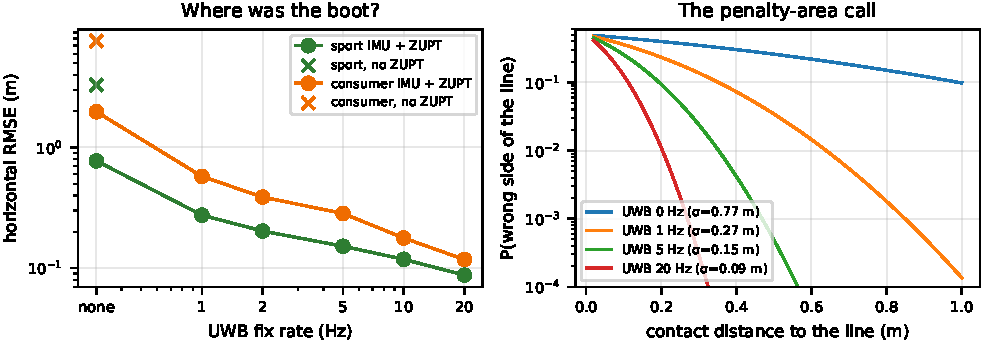
\includegraphics[width=\textwidth]{figures/localize.pdf}
\caption{Left: horizontal position RMSE of the boot over the second half of a
\LocDuration\,s run with a cut, versus ultra-wideband fix rate, for an
impact-rated and a phone-grade IMU with zero-velocity updates (crosses: free
inertial integration). Right: probability of placing a contact on the wrong
side of a line versus its distance to the line, for several fix rates.}
\label{fig:localize}
\end{figure*}

Ordering the contacts says whether a foul happened; placing it says where the
free kick is taken and whether it is a penalty. Figure~\ref{fig:localize}
gives the boot's position error from its own IMU with zero-velocity updates
(ZUPT) and sparse ultra-wideband (UWB) fixes, over \LocNRuns\ runs. Free
inertial integration drifts to \LocFreeSport\,m (sport IMU) and
\LocFreeCons\,m (consumer) horizontally within a few seconds; ZUPT alone brings
this to \LocZuptSport\,m and \LocZuptCons\,m, because every stance resets
velocity and drift accumulates per stride rather than per second
\cite{foxlin2005pedestrian}. One UWB fix per second is worth more than the
IMU grade: \LocUwbOneSport\,m for the sport part, and at 10\,Hz
\LocUwbTenSport\,m, at 20\,Hz \LocUwbTwentySport\,m (consumer:
\LocUwbTwentyCons\,m) --- close to the \LocUwbSigma\,m of the anchors
themselves, at which point the filter is interpolating between fixes with the
IMU rather than dead-reckoning.

Read as a decision, the right panel is the penalty-area call. With 10\,Hz
fixes a contact 25\,cm outside the line is placed inside with probability
\LocWrongQuarterTen\%, at 10\,cm the probability is \LocWrongTenTen\%, and at
50\,cm it is below $0.01$\%; with ZUPT alone the 50\,cm case is wrong
\LocWrongHalfZupt\% of the time. This is the same logic as the timing result:
there is a resolution (about $\sigma_{\text{pos}}$ in space, about one pulse
duration in time) inside which the sensors return a probability near one
half, and outside which they return a confident answer. Note that the boot's
position is a proxy: the foul's location is the contact point, which is
within a boot length of the sensor, and the penalty-area rule concerns the
\emph{offence} location, so the same $\Phi(-d/\sigma)$ applies with $d$
measured from that point.
